\title{Chapter 2: Multi-armed Bandits - Exercises}


\author{Jacob Taylor Cassady}

\documentclass{article}
\usepackage{textcomp}
\usepackage{textgreek}
\usepackage{bbding, pifont}
\usepackage{graphicx}
\graphicspath{ {.} }

\begin{document}

\maketitle

\section{In \textepsilon-greedy action selection, for the case of two actions and \textepsilon \thickspace = 0.5, what is the probability that the greedy action is selected?}
50 percent.

\section{Bandit example}
Consider a k-armed bandit problem with k = 4 actions, denoted 1, 2, 3, and 4. 
Consider applying to this problem a bandit algorithm using \textepsilon-greedy action selection, 
sample-average action-value estimates, and initial estimates of $ Q_1(a) $ = 0, for all \emph{a}. 
Suppose the initial sequence of actions and rewards is $A_1$ = 1, $R_1$ = \textminus 1, $A_2$ = 2, 
$R_2$ = 1, $A_3$ = 2, $R_3$ = \textminus 2, $A_4$ = 2, $R_4$ = 2, $A_5$ = 3, $R_5$ = 0. 
On some of these time steps the \textepsilon \thickspace case may have occurred, causing an action 
to be selected at random.

\paragraph{See Figure 1 at the end of the document for the output of the code I wrote for this.}

\begin{figure}[b]
    \centering
    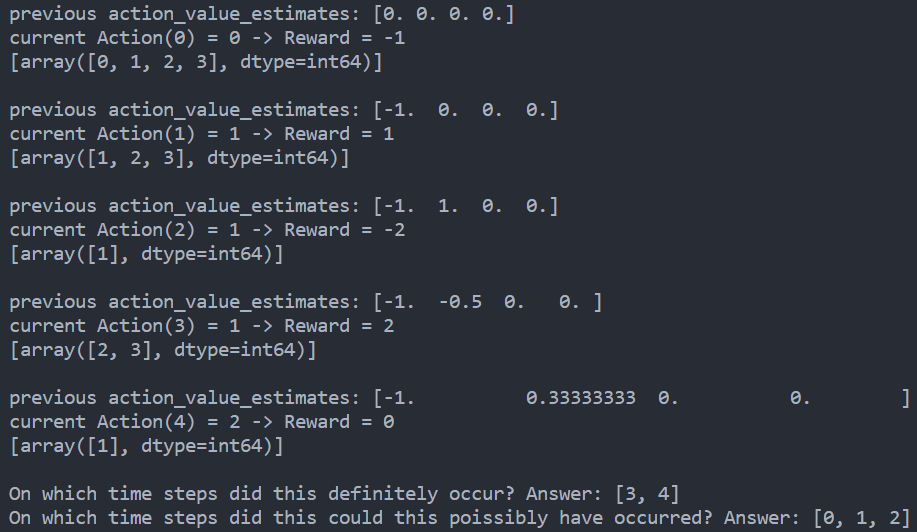
\includegraphics{bandit_example_output.png}    
    \caption{Output of bandit\_example.py}
\end{figure}

\subsection{On which time steps did this definitely occur?}
Note. I am indexing the time steps by 0. Answer: [3, 4]
\subsection{On which time steps could this possibly have occurred?}
Note. I am indexing the time steps by 0. Answer: [0, 1, 2]

\section{In the comparison shown in Figure 2.2, }
Express your answer quantitatively.
\subsection{which method will perform best in the long run in terms of cumulative reward and probability
            of selecting the best action?}
\textepsilon=0.01
\subsection{How much better will it be?}
\textepsilon=0.1 would perform at best 91\% optimal. \textepsilon=0.01 would perform at best 99.1\% optimal. After convergence, \textepsilon=0.01 would perform 8.1\% better.

\section{If the step-size parameters, $\alpha_n$, are not constant, then the estimate $Q_n$ is a weighted average of previously received rewards with a weighting different from that given by (2.6).}
\subsection{What is the weighting on each prior reward for the general case, analogous to (2.6), in terms of the sequence of step-size parameters?}

\section{programming}
\paragraph{Design and conduct an experiment to demonstrate the difficulties that sample-average methods have for nonstationary problems. Use a modified version of the 10-armed testbed in which all the $q_*(a)$ start out equal and then take independent random walks (say by adding a normally distributed increment with mean zero and standard deviation 0.01 to all the $q_*(a)$ on each step). Prepare plots like Figure 2.2 for an action-value method using sample averages, incrementally computed, and another action-value method using a constant step-size parameter, \textalpha \thickspace = 0.1. Use \textepsilon \thickspace = 0.1 and longer runs, say of 10,000 steps.}

\section{Mysterious Spikes}

\section{Unbiased Constant-Step-Size Trick}

\section{UCB Spikes}

\section{Show that in the case of two actions, the soft-max distribution is the same as that given by the logistic, or sigmoid, function often used in statistics and artificial neural networks.}

\section{Suppose you face a 2-armed bandit task whose true action values change randomly from time step to time step. Specifically, suppose that, for any time step, the true values of actions 1 and 2 are respectively 0.1 and 0.2 with probability 0.5 (case A), and 0.9 and 0.8 with probability 0.5 (case B).}
\subsection{If you are not able to tell which case you face at any step, what is the best expectation of success you can achieve and how should you behave to achieve it?}
\subsection{Now suppose that on each step you are told whether you are facing case A or case B (although you still don't know the true action values). This is an associative search task. What is the best expectation of success you can achieve in this task, and how should you behave to achieve it?}

\section{programming}
\paragraph{Make a figure analogous to Figure 2.6 for the nonstationary case outlined in Exercise 2.5. Include the constant-step-size \textepsilon-greedy algorithm with \textalpha=0.1. Use runs of 200,000 steps and, as a performance measure for each algorithm and parameter setting, use the average reward over the last 100,000 steps.}

\end{document}
